\lab{Applications}{SVD decomposition}{SVD decomposition}

\objective{Explore applications of the SVD, an important matrix factorization algorithm.}

Now we're going to briefly discuss the singular value decomposition and how it can be used to implement a very simple form of lossy image compression. Recall that the SVD is a decomposition of the $m\times n$ matrix $A$
of rank $r$ into the product $A = U \Sigma V^H$, where $U$ and $V$
are unitary matrices having dimensions $m\times m$ and $n\times n$,
respectively, and $\Sigma$ is the $m\times n$ diagonal matrix
\[
\Sigma = \mbox{diag}(\sigma_1,\sigma_2,\ldots,\sigma_r,0,\ldots,0),
\]
where $\sigma_1 \geq \sigma_2 \geq \ldots \geq \sigma_r > 0$ are the
singular values of $A$.  Upon closer inspection, we can write
\[
U = \begin{pmatrix}U_1 & U_2\end{pmatrix}, \quad \Sigma =
\begin{pmatrix}\Sigma_r & 0\\0 & 0\end{pmatrix}, \quad V =
\begin{pmatrix}V_1 & V_2\end{pmatrix},
\]
where $U_1$ and $V_1$ have dimensions $m\times r$ and $n\times r$
respectively and $\Sigma_r$ is the $r\times r$ diagonal matrix of
(nonzero) singular values.  Multiplying this out yields the reduced
form of the SVD
\[
A =
\begin{pmatrix}U_1 & U_2\end{pmatrix}
\begin{pmatrix}\Sigma_r & 0\\0 & 0\end{pmatrix}
\begin{pmatrix}V^H_1 \\ V^H_2\end{pmatrix} =
U_1 \Sigma_r V_1^H
\]
\subsection{Low rank data storage}

If the rank of a given matrix is significantly smaller than its
dimensions, the reduced form of the SVD offers a way to store the
matrix with less memory.  As it is, the $m\times n$ matrix requires
the storage of $mn$ numbers, whereas $U_1$, $\Sigma_r$ and $V_1$ in
the reduced form of the SVD, all together require $r(m+n+1)$ numbers
(verify this).  Thus if $r$ is much smaller than both $m$ and $n$,
we can obtain considerable efficiency.  As an example, suppose
$m=100$, $n=200$ and $r=20$. Then the original matrix requires
20,000 numbers for storage whereas the reduced form of the SVD only
requires 6020 numbers.

\subsection{Low rank approximation}

The reduced form of the SVD also provides a way to approximate a
matrix with one of lower rank. This idea hits many areas of applied
mathematics, including signal processing, statistics, semantic
indexing (search engines), and control theory.  Given a matrix $A$,
we can find an approximate matrix $\widehat A$ of rank $r$ by taking
the SVD of $A$ and setting all of its singular values after
$\sigma_r$ to zero, that is,
\[
\sigma_{r+1} = \sigma_{r+2} = \cdots = \sigma_n = 0,
\]
and then multiplying the matrix back together again.  How to know how much rank
to keep?  Try plotting the the singular values.  We have plotted the singular values to the image below.  Matrix rank is on the x-axis and the eigenvalues are the y-axis.  Note that SVD decomposition orders the eigenvalues from greatest to least.  The greatest eigenvalues contribute most to the image while the smallest eigenvalues hardly contribute anything.  By looking at the graph we can see how many eigenvalues we need to use to maintain good quality.  The matrix rank of image is $670$.  However, as the plot shows, we could easily reduce the rank in half without have any noticable effect on image quality.

\begin{center}
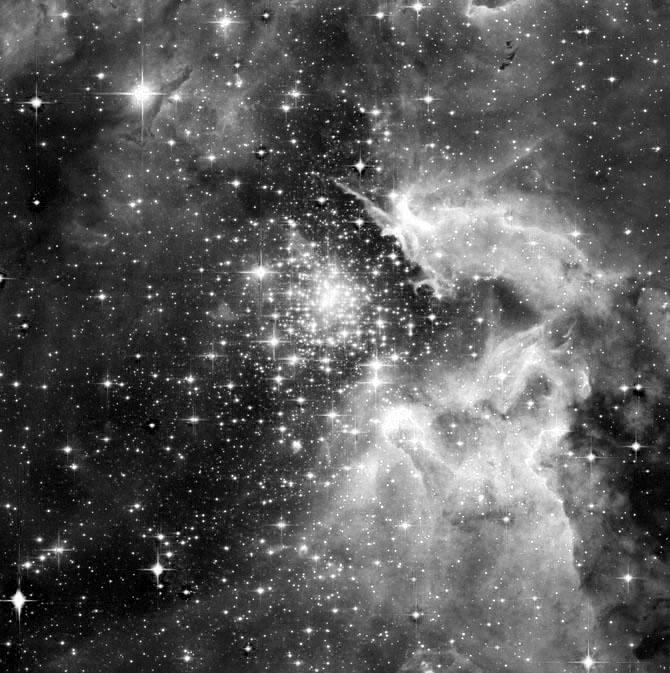
\includegraphics[scale=.2]{./Figures/hubble_red.png}

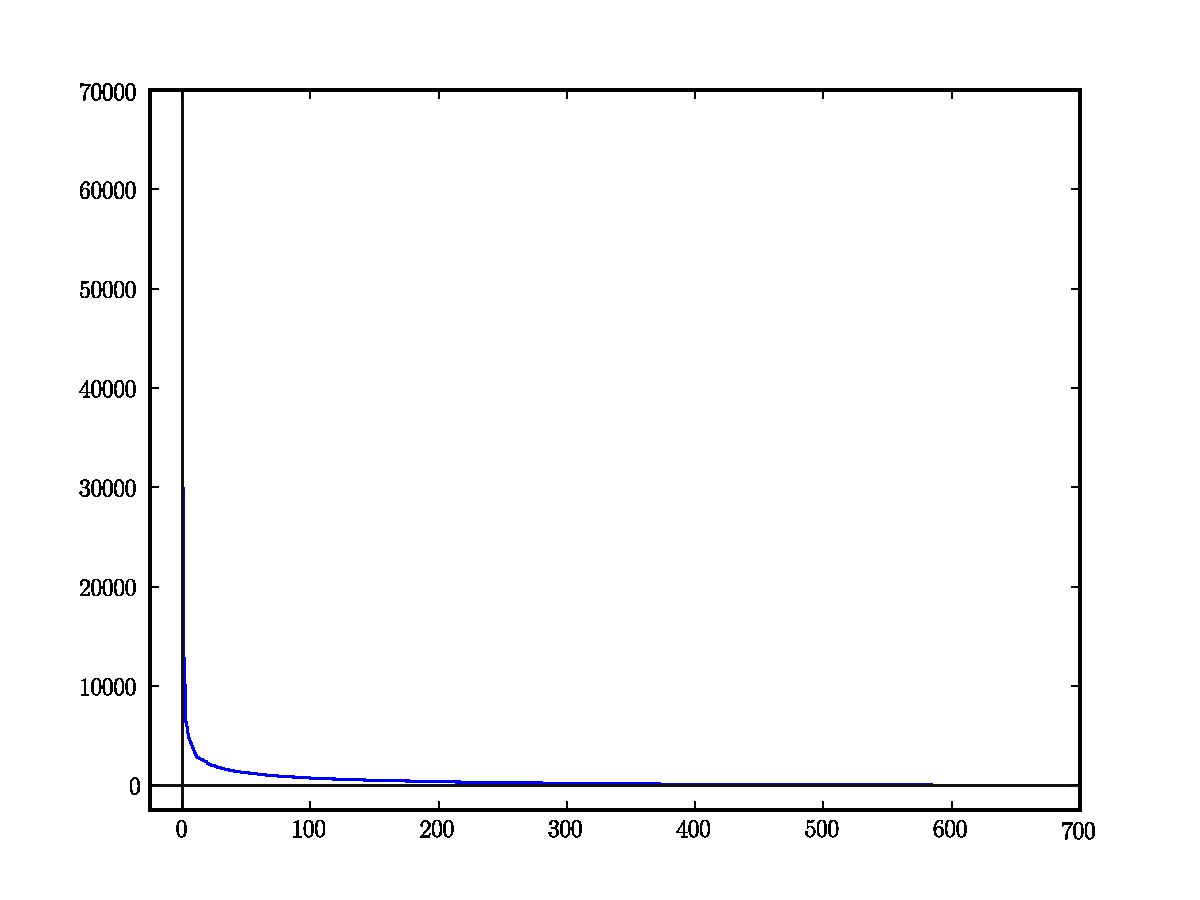
\includegraphics[scale=.4]{./Figures/hubble_svals.pdf}
\end{center}

\begin{matlab}
 \begin{lstlisting}[style=matlab]
>> A = [1 1 3 4; 5 4 3 7; 9 10 10 12; 13 14 15 16; 17 18 19 20]
>> rank(A)
>> [U,S,V] = svd(A)
>> Ahat = U(:,1:3)*S(1:3,1:3)*V(:,1:3)'
>> rank(Ahat)
\end{lstlisting}[style=matlab]
\end{matlab}
\begin{python}
\begin{lstlisting}[style=python]
: import scipy as sp
: import scipy.linalg as la
: A = sp.array([[1,1,3,4],[5,4,3,7],[9,10,10,12],[13,14,15,16],[17,18,19,20]])
: sp.np.linalg.matrix_rank(A)
: U,s,Vt = la.svd(A)
: S = sp.zeros(A.shape)
: S[0:s.size,0:s.size)] = sp.diag(s)
: Ahat = sp.dot(sp.dot(U[:,0:2], S[0:2,0:2]), Vt[0:2,:])
\end{lstlisting}

We can compute the rank of a matrix by looking at the number of nonzero singular values in the SVD decompositon.  The following function will compute the rank of a matrix.  The \li{sp.finfo(float).eps} tells us the smallest representable postitive number such that $1.0+\mbox{eps} != 1.0$  Anything smaller than the eps value is numerically zero to the computer.
\begin{lstlisting}[style=python]
: def matrix_rank(X):
:.... S = la.svd(X, compute_uv=False)
:.... tol = S.max()*sp.finfo(S.dtype).eps
:.... return sum(S>tol)
: matrix_rank(Ahat)
\end{lstlisting}
\end{python}
Note that $\widehat A$ is ``close'' to the original matrix $A$, but
that its rank is 3 instead of 4.

\subsection{Application to Imaging}

\begin{matlab}
 Enter the following into MATLAB:
\begin{lstlisting}[style=matlab]
>> load('clown.mat');
>> image(X);
>> colormap(map); axis off;
\end{lstlisting}
The image \li{X} is a $200\times 320$ matrix (type \li{size(X)}
into MATLAB's command line).  The numbers range from $1$ to $81$ and
correspond to different shades of gray.  We compute the SVD of our
image \li{X} by executing
\begin{lstlisting}[style=matlab]
>> [U,S,V] = svd(X);
\end{lstlisting}
Note that the rank of \li{X} is 200.  We can reduce our clown image
to a rank of 50 by executing the following:
\begin{lstlisting}[style=matlab]
>> n=50;
>> Xhat = U(:,1:n)*S(1:n,1:n)*V(:,1:n)';
>> image(Xhat);
\end{lstlisting}
Note that the clown's left cheek is a little blurry, but it
otherwise looks ok.  How low can you take the rank and still have a
decent looking image?  What happens when you take the rank too low?

\begin{problem}
Explore the clown picture for several different values of rank.
Conduct the experiments described above.  Note that the original
image takes 64,000 integers to store.  Compare this with the storage
needs for various lower-rank SVD approximations. What conclusions
can you draw? Experiment with other images included in MATLAB to see how it works in other cases.
\end{problem}
\end{matlab}

\begin{python}
Enter the following into Python (note that any image you might have will work):
\begin{lstlisting}
: import matplotlib.pyplot as plt
: X = sp.misc.imread('fingerprint.png')
: sp.misc.imshow(X)
\end{lstlisting}
Computing the SVD of your image is simple.  Remember to make the singluar values a diagonal matrix before multiplying.
\begin{lstlisting}
: U,s,Vt = la.svd(X)
: S = sp.diag(s)
\end{lstlisting}
In the next code block, $n$ repsents the desired rank of the output.
\begin{lstlisting}
: n=50;
: Xhat = sp.dot(sp.dot(U[:,0:n], S[0:n,0:n]), Vt[0:n,:])
: sp.misc.imshow(Xhat)
\end{lstlisting}

%write code that will caluculate final image column by column in rank 1 approximations.  It is actually smaller to transmit the matrix col by col than chunks of cols.  We only send 70% of the data if we send col by col than entire matices.  1017856bytes vs 1445888 bytes.
\begin{problem}
A law enforcement agency has been needing to efficiently store over 50,000 fingerprints.  They have decided to use the SVD compression algorithm.  Your job is to try several parameters for SVD algorithm and recommend the those parameters that retain the highest quality but compress the most.  There should be no smearing or blocking in the final image and fingerprint detail must be retained (otherwise the fingerprint is worthless).  As part of your recommendation, calculate how much hard disk space would be needed to store each compressed fingerprint.
\end{problem}
% \begin{problem}
% Explore the clown picture for several different values of rank.
% Conduct the experiments described above.  Note that the original
% image takes 64,000 integers to store.  Compare this with the storage
% needs for various lower-rank SVD approximations. What conclusions
% can you draw? Expirement with other images we've used in this book.
% \end{problem}
\end{python}
